% =============================================================================
% sections/07_science_geology.tex  -  Section 7: Science - Regional Geology Analysis
% Teams: science (Bohdan) / Status: draft
%
% SCORING (0-10 pts). Two pages A4 total:
%   1) COMPOSITE MAP on one A4:
%      a) location map of the landing site at global scale
%      b) regional geological map (Astrogeology Science Centre publications)
%      c) close-up map (CTX or HiRISE) with: landing ellipse, planned rover
%         path, three regions of interest
%   2) REPORT, up to 800 words: technical justification (why it is safe to
%      land) + scientific justification (why it is worth landing, especially
%      w.r.t. the three ROIs).
%
% CONSTRAINTS for site selection: geologically interesting within a rover
%   traverse of up to 30 km; landable with current techniques (atmospheric
%   thickness, landing area); safe for the rover (local slopes < 20 deg, few
%   large boulders, survivable winter thermal conditions).
% TOOLS: Google Earth Pro (Mars) or JMars.
% =============================================================================

\section{Science: Regional Geology Analysis}
\label{sec:science_geology}

The composite regional geology map is shown in \autoref{fig:regional_geology_map_placeholder} and is intended to present the landing-site context, the regional geological setting, and the planned rover traverse.

\begin{figure}[p]
  \centering
  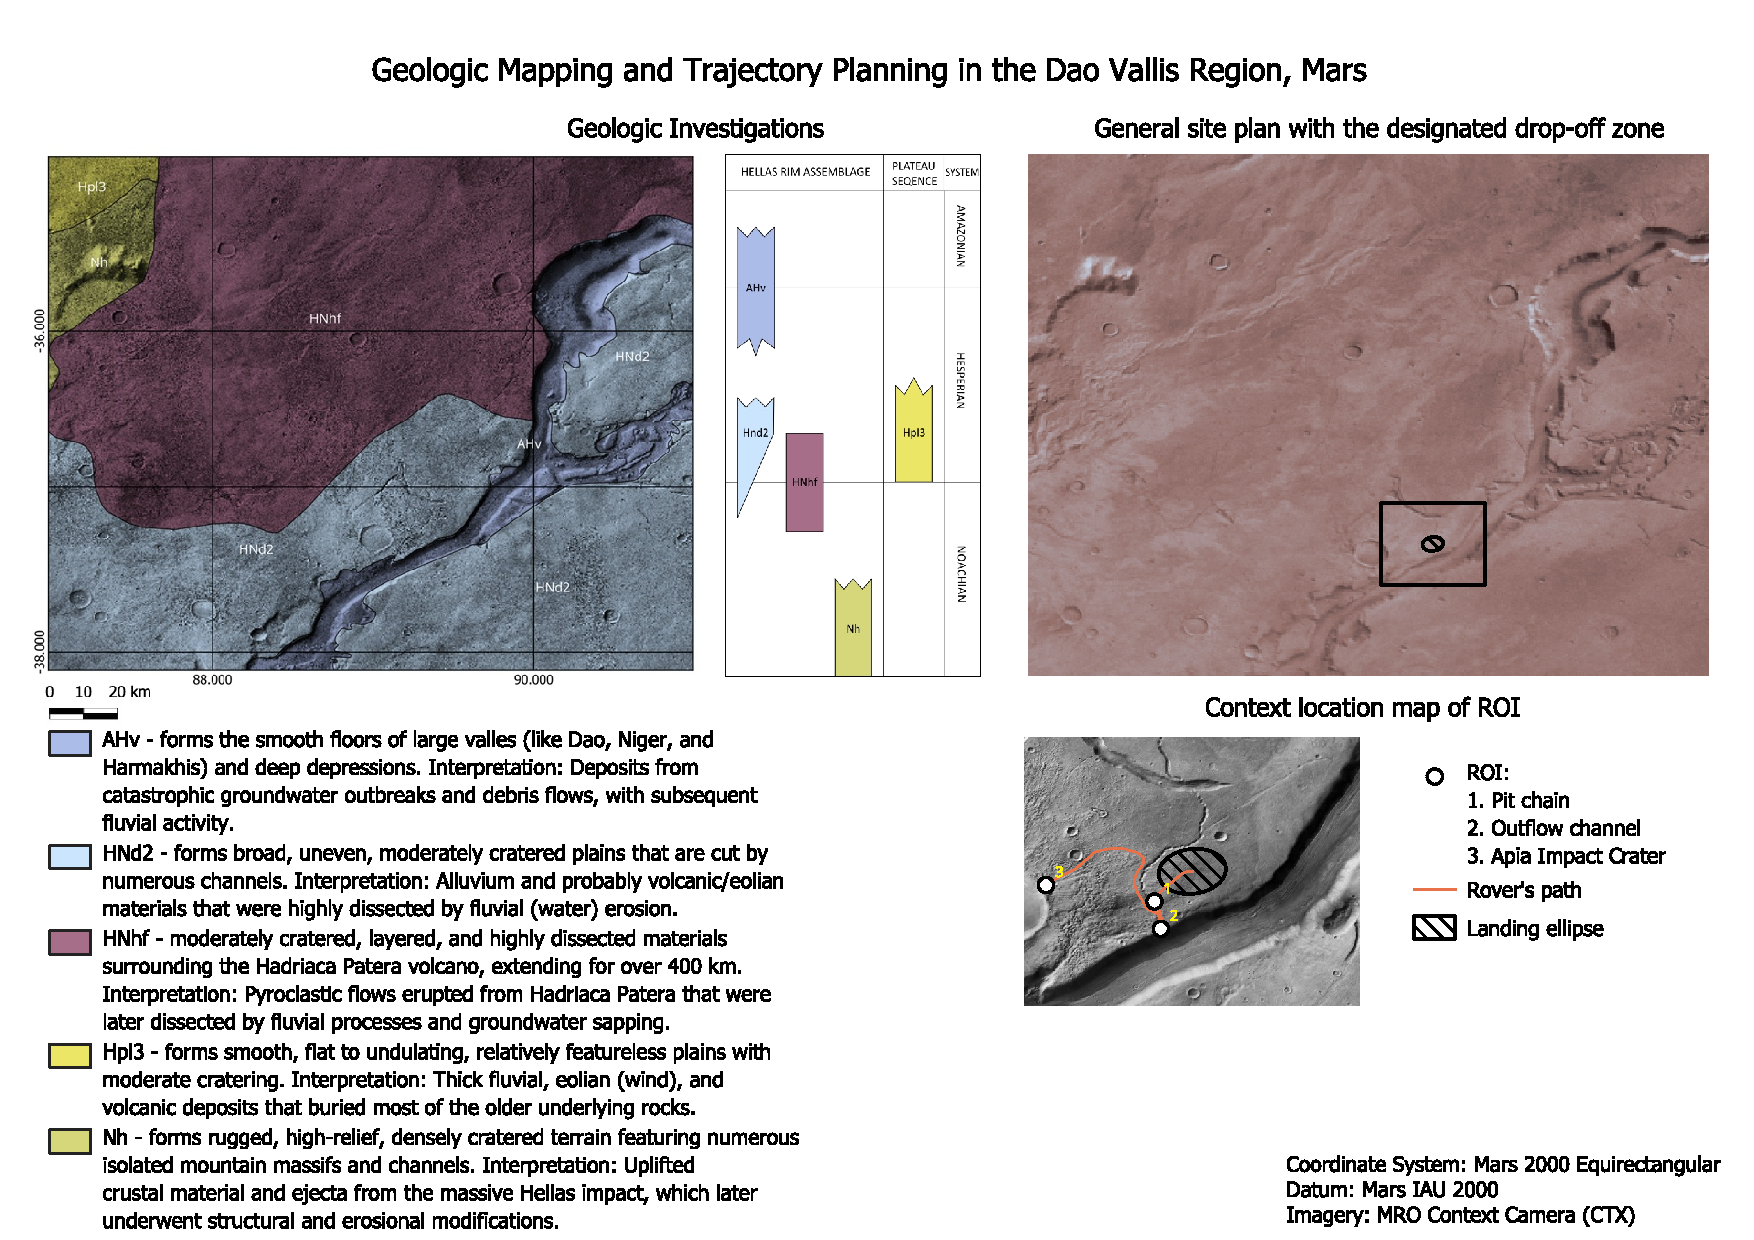
\includegraphics[page=1,width=\textwidth,height=0.92\textheight,keepaspectratio]{teams/science/figures/regional_geology_map.pdf}
  \caption{Placeholder for the composite regional geology map PDF.}
  \label{fig:regional_geology_map_placeholder}
\end{figure}

\subsection{Geological Characterization of the Region}
\label{sec:geological_characterization}

\subsubsection{General Characterization}
\label{sec:general_characterization}
\todo[inline]{Add a concise summary of Hellas Planitia, Dao Vallis, and the main geological units.}

Hellas Planitia is a broad impact basin on Mars with a smooth floor, extensive crater modification, and evidence of later sedimentary and erosional overprint. Dao Vallis is one of the most prominent channel systems associated with the basin and is commonly interpreted as a landform shaped by fluid flow, either as a transient discharge route or as part of a longer erosional history. The surrounding terrain combines plains, depressions, and local rises, making the region a useful archive of both basin evolution and surface modification. The basin setting also preserves important clues about the interaction between impact processes, deposition, and later modification by water or ice.

\subsubsection{Scientific Potential of the Region}
\label{sec:scientific_potential}
\todo[inline]{Add a brief explanation of why the site is scientifically valuable.}

The site is attractive because it links regional basin history with local evidence of fluid activity. Its morphology can help constrain the timing of channel incision, the role of water in shaping the terrain, and the relationship between local relief and wider geological processes. The presence of possible structural lineaments and depressions provides a strong basis for testing whether the landscape reflects water erosion, tectonic modification, or a combination of both. For this reason, the region can address both local questions about channel formation and broader questions about the geological evolution of the Hellas basin.

\subsection{Landing Site Selection Rationale}
\label{sec:landing_site_selection}

\subsubsection{Candidate Analysis}
\label{sec:candidate_analysis}
\todo[inline]{Add the five candidate ellipses and the evaluation criteria.}

Five landing ellipses were considered around Dao Vallis. Each candidate was assessed against the same criteria: slope, elevation contrasts, roughness, distance to high-value geology, and accessibility for a rover traverse. The best options were those that combined safe operations with access to landforms that could test the main scientific hypothesis. Less favorable ellipses were rejected because they offered poorer terrain conditions, more hazardous relief, or weaker links to the key geological targets. The comparison therefore focused on balancing engineering safety with scientific return.

\subsubsection{Final Landing Ellipse Selection}
\label{sec:final_landing_ellipse}
\todo[inline]{Explain the final choice and the reasons for rejecting the others.}

The selected ellipse is preferred because it offers the most balanced combination of safety and scientific return. It lies close to the most informative terrain while remaining within operational limits for slope and roughness. The rejected ellipses were either too close to hazardous relief, too far from the main geomorphological targets, or insufficiently representative of the processes that shaped Dao Vallis. This choice therefore maximizes the probability of successful operations while preserving access to the most valuable geology.

\subsection{Mission Scientific Hypothesis}
\label{sec:scientific_hypothesis}
\todo[inline]{Refine the core hypothesis and connect it to the expected observations.}

The working hypothesis is that Dao Vallis formed through the interaction of liquid water and basin-scale structural evolution. In this interpretation, channel incision and the nearby linear depressions reflect a shared geological history involving fluid flow, collapse, and later modification. If the hypothesis is correct, rover observations should reveal signatures of erosion, structural control, and a clear relationship between local morphology and the wider Hellas basin history. The hypothesis is therefore directly testable through surface observations and targeted traverse planning.

\subsection{Geological Investigation Plan}
\label{sec:investigation_plan}

\subsubsection{Selection of Regions of Interest}
\label{sec:roi_selection}
\todo[inline]{Define the regions of interest and justify their selection.}

Three regions of interest will be prioritized. The first will focus on the main channel morphology and evidence for flow direction. The second will target possible structural depressions or lineaments that may indicate tectonic influence. The third will examine the surrounding plains to place the local landforms within the larger basin context. This arrangement maximizes the range of geological evidence while keeping the traverse compact and efficient. Each ROI is selected to address a different part of the same scientific story.

\subsubsection{Route Plan}
\label{sec:route_plan}
\todo[inline]{Describe the order of visits and the logic of the route.}

The route will begin with the safest and most accessible targets before moving to more complex terrain. This ordering limits unnecessary driving, saves energy, and ensures that the highest-value observations are collected early. It also allows the rover to test the main geological hypotheses while preserving enough mobility for follow-up investigations near the most promising landforms. The plan is intentionally conservative in its first phase and more ambitious in its later phase.

\subsection{Expected Results}
\label{sec:expected_results}
\todo[inline]{Summarize the expected outcomes of the mission.}

The mission is expected to clarify the origin of the linear depressions associated with Dao Vallis, test the role of water-related erosion in shaping the landscape, and refine the geological history of the Hellas basin. The results will also verify whether the selected landing ellipse is well matched to the scientific goals of the mission and whether the proposed hypothesis is supported by direct observations. In the best case, the investigation will provide a coherent picture of how fluid processes and structural evolution combined to shape the region.
